\documentclass[11pt]{article}
\usepackage[letterpaper,margin=0.72in]{geometry}
\usepackage[T1]{fontenc}
\usepackage{lmodern}
\usepackage{microtype}
\usepackage{amsmath,amssymb,mathtools}
\usepackage{booktabs,longtable,array,tabularx}
\usepackage{enumitem}
\usepackage{xcolor}
\usepackage{hyperref}
\usepackage{listings}
\usepackage{fancyhdr}
\usepackage{titlesec}
\usepackage{tikz}
\usetikzlibrary{arrows.meta,positioning,shapes.geometric,fit,calc,backgrounds}
\usepackage{float}
\usepackage{caption}
\usepackage{verbatim}

\definecolor{navy}{HTML}{17365D}
\definecolor{teal}{HTML}{1F6D72}
\definecolor{gold}{HTML}{A57418}
\definecolor{softblue}{HTML}{EAF2F8}
\definecolor{softgreen}{HTML}{EAF7EF}
\definecolor{softgold}{HTML}{FBF3DF}
\definecolor{softred}{HTML}{FBEAEA}
\definecolor{codegray}{HTML}{F5F5F5}
\definecolor{darkgray}{HTML}{555555}

\hypersetup{colorlinks=true,linkcolor=navy,urlcolor=teal,citecolor=navy,pdfauthor={for Brian Tenneson},pdftitle={Predator 8.018 Reconstruction and Resume Notes}}
\pagestyle{fancy}
\fancyhf{}
\lhead{Predator 8.018 Reconstruction Notes}
\rhead{for Brian Tenneson}
\cfoot{\thepage}
\setlength{\headheight}{14pt}
\setlist[itemize]{leftmargin=1.45em,itemsep=0.25em,topsep=0.35em}
\setlist[enumerate]{leftmargin=1.55em,itemsep=0.25em,topsep=0.35em}
\titleformat{\section}{\Large\bfseries\color{navy}}{\thesection}{0.7em}{}
\titleformat{\subsection}{\large\bfseries\color{teal}}{\thesubsection}{0.65em}{}
\titleformat{\subsubsection}{\normalsize\bfseries\color{gold}}{\thesubsubsection}{0.6em}{}

\lstset{
  basicstyle=\ttfamily\small,
  backgroundcolor=\color{codegray},
  frame=single,
  rulecolor=\color{gray!35},
  breaklines=true,
  columns=fullflexible,
  showstringspaces=false,
  aboveskip=0.7em,
  belowskip=0.7em
}

\newcommand{\code}[1]{\texttt{#1}}
\newcommand{\Hhat}{\widehat H}
\newcommand{\Rcost}{R}
\newcommand{\accept}{\mathrm{ACCEPT}}

\begin{document}

\begin{titlepage}
\centering
\vspace*{0.65in}
{\Huge\bfseries\color{navy} Predator 8.018 Reconstruction\par}
\vspace{0.15in}
{\Huge\bfseries\color{navy} and Resume Notes\par}
\vspace{0.35in}
{\Large Settlement Geometry, Proof Compass Control,\par}
{\Large Self-Aware Bailout, and Selective Kitchen-Sink Roadmap\par}
\vspace{0.6in}
{\LARGE\bfseries for Brian Tenneson\par}
\vspace{0.35in}
{\large Technical snapshot: August 26, 2026\par}
\vspace{0.12in}
{\large Repository: \code{btenneson/ATP}\par}
{\large Frozen reconstruction commit: \code{77aad00387b459b05da35abaea5e43d2fbd0a6db}\par}
\vfill
\begin{minipage}{0.88\textwidth}
\small
\textbf{Purpose.} These are not publication notes. They are restart/reconstruction notes intended to make it possible to resume the experiment after loss of conversational context, provided the repository and named runtime/model/data files are available. They distinguish (i) what is implemented and tested, (ii) what is mathematically proved but not enforced by the controller, and (iii) what was planned as the next selective kitchen-sink implementation.
\end{minipage}
\vfill
\end{titlepage}

\tableofcontents
\newpage

\section{Executive restart summary}

The immediate research question is not whether a heuristic score looks good. The operational question is:
\[
\boxed{\text{Does settlement-distance control produce a verified settlement within budget, and how quickly?}}
\]
The intended performance quantity is first settlement resource:
\[
\tau_0=\inf\{R:H(A_R)=0\}.
\]
The current experimental line uses the Metamath theorem \code{prcom} as the target and a recovered Predator 8.002 lineage. The current implemented version at this snapshot is \textbf{Predator 8.018}, which adds a first concrete self-awareness rule: a promising proof-tree basin receives only a bounded resource tranche; if cost continues without meaningful benefit, the controller blacklists that basin and deliberately moves elsewhere.

The essential conceptual progression is:
\[
\boxed{\text{move search} \to \text{measure progress} \to \text{judge strategy} \to \text{change strategy if cost/benefit collapses}.}
\]

At the moment of this document snapshot, GitHub Actions run \code{32966066334}, workflow \code{Predator8 prcom self-aware bailout}, was still \textbf{in progress}. Do not infer a result from these notes; query the workflow or its artifact before resuming.

\subsection{The single most important rule}

The verifier remains authoritative. Every heuristic, partial-credit score, learned rank, imagination signal, basin score, exactification hint, Professor decision, or self-awareness judgment is non-authoritative. A theorem is settled only when the proof certificate verifies.

\section{Three layers of the system}

The present architecture is easiest to reconstruct as three nested control levels.

\begin{figure}[H]
\centering
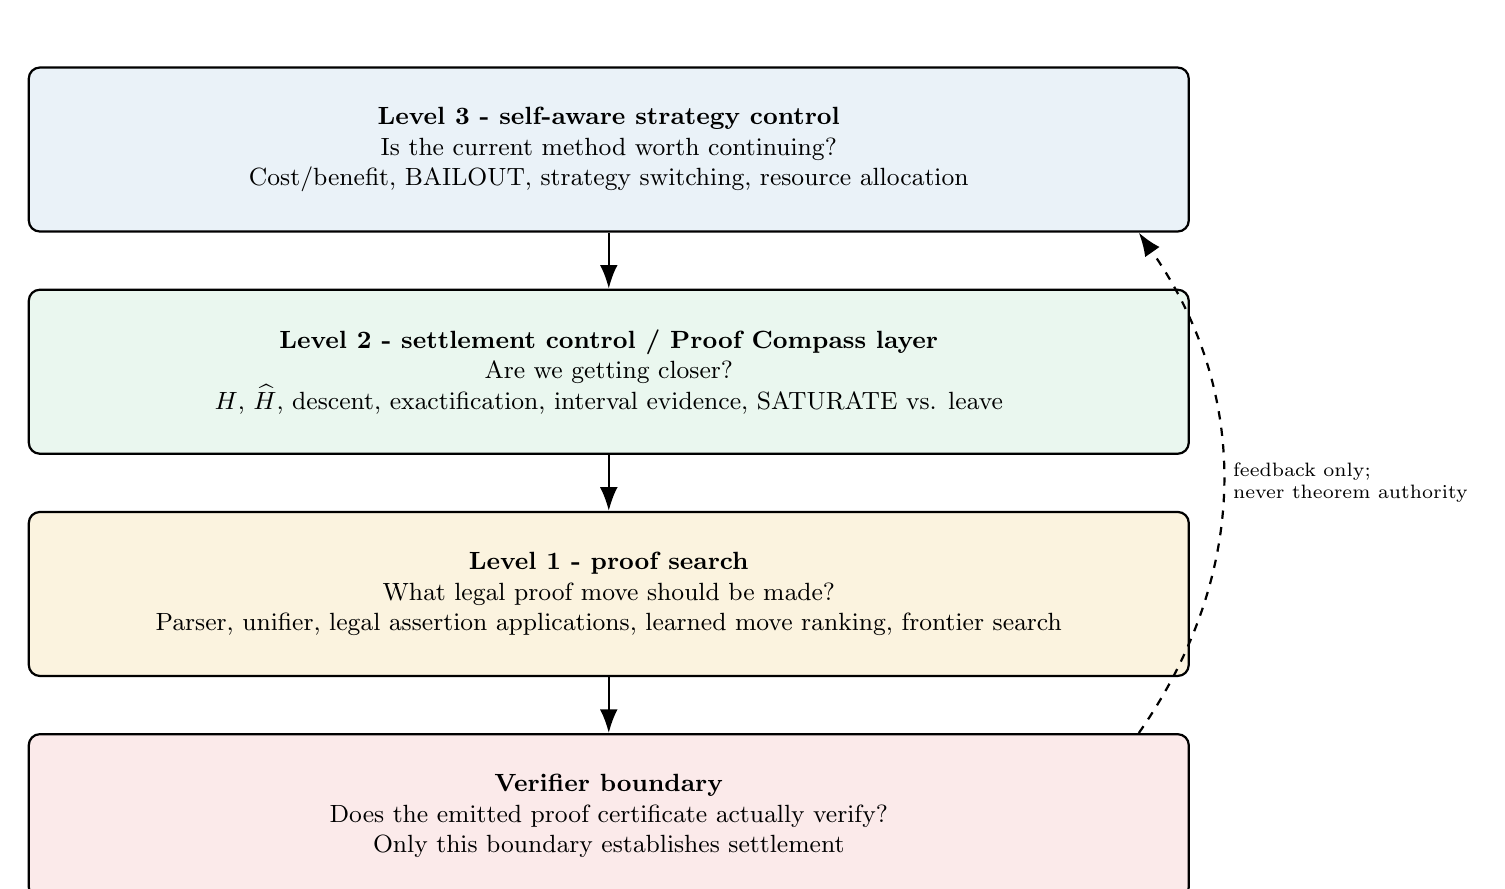
\begin{tikzpicture}[
  box/.style={draw,rounded corners,thick,minimum width=5.8in,minimum height=0.82in,align=center,font=\small},
  arr/.style={-{Latex[length=3mm]},thick}
]
\node[box,fill=softblue] (l3) {\textbf{Level 3 - self-aware strategy control}\\Is the current method worth continuing?\\Cost/benefit, BAILOUT, strategy switching, resource allocation};
\node[box,fill=softgreen,below=0.28in of l3] (l2) {\textbf{Level 2 - settlement control / Proof Compass layer}\\Are we getting closer?\\$H$, $\widehat H$, descent, exactification, interval evidence, SATURATE vs. leave};
\node[box,fill=softgold,below=0.28in of l2] (l1) {\textbf{Level 1 - proof search}\\What legal proof move should be made?\\Parser, unifier, legal assertion applications, learned move ranking, frontier search};
\node[box,fill=softred,below=0.28in of l1] (v) {\textbf{Verifier boundary}\\Does the emitted proof certificate actually verify?\\Only this boundary establishes settlement};
\draw[arr] (l3) -- (l2);
\draw[arr] (l2) -- (l1);
\draw[arr] (l1) -- (v);
\draw[arr,dashed] ([xshift=2.65in]v.north) to[bend right=35] node[right,font=\scriptsize,align=left]{feedback only;\\never theorem authority} ([xshift=2.65in]l3.south);
\end{tikzpicture}
\caption{The intended hierarchy. Predator 8.018 implements only an early, simple Level-3 rule.}
\end{figure}

The research aspiration is eventually to make strategy judgment stronger than human mathematical metareasoning. The present milestone is more modest: \emph{make the machine notice when effort is buying almost nothing and stop sinking resources into quicksand.}

\section{Formal settlement geometry}

\subsection{Exact settlement horizon}

Fix the legal proof-state graph. Let $q$ be a proof state and let $\accept$ be the verifier-accepted terminal state. The exact unit-cost settlement horizon is
\[
H(q)=d(q,\accept)\in\mathbb N_0\cup\{\infty\}.
\]
In the unit-edge geometry:
\[
H(q)=0\iff q=\accept.
\]
If $0<H(q)<\infty$, a geodesic successor $q'$ satisfies
\[
H(q')=H(q)-1.
\]

\subsection{First-settlement objective}

The controller uses $H$ to navigate, but the experiment is ultimately judged by the first resource time at which settlement occurs:
\[
\boxed{\tau_0=\inf\{R:H(A_R)=0\}.}
\]
For a budget $B$, classify behavior operationally as:
\begin{center}
\begin{tabular}{ll}
\toprule
Condition & Interpretation \\
\midrule
$\tau_0\ll B$ & quick settlement \\
$\tau_0\lesssim B$ & barely within budget \\
$\tau_0>B$ or no certificate & no settlement within declared budget \\
\bottomrule
\end{tabular}
\end{center}

\subsection{The implemented heuristic is not exact $H$}

The recovered controller currently uses a simple non-authoritative heuristic $\widehat H$ from Predator 8.015:
\[
\widehat H
=1+\#\text{goals}
+0.015\,(\text{token count})
+0.02\tanh\!\left(\frac{\#\text{metavariables}}{8}\right),
\]
with $\widehat H=0$ for a state with no open goals.

This is crucial: a plateau near $\widehat H\approx2.03$ does \textbf{not} imply that true $H=2$. The 8.016/8.017 experiments demonstrated precisely why estimated proximity needs certification.

\section{Proof tree orientation and the ``barking down a tree'' picture}

Backward theorem proving begins at a target goal and expands downward into possible proof decompositions. A verified closed proof is a leaf (or terminal path) below the root.

\begin{figure}[H]
\centering
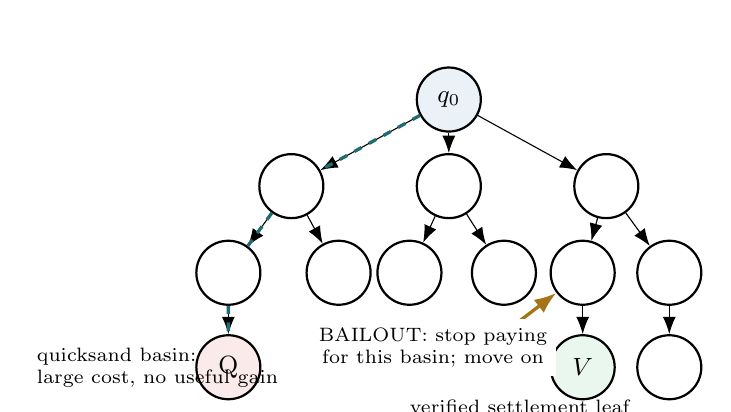
\begin{tikzpicture}[
  every node/.style={font=\small},
  state/.style={circle,draw,thick,minimum size=0.32in,inner sep=1pt},
  good/.style={state,fill=softgreen},
  bad/.style={state,fill=softred},
  arr/.style={-{Latex[length=2.2mm]},thin}
]
\node[state,fill=softblue] (r) at (0,0) {$q_0$};
\node[state] (a) at (-2,-1.1) {};
\node[state] (b) at (0,-1.1) {};
\node[state] (c) at (2,-1.1) {};
\node[state] (a1) at (-2.8,-2.2) {};
\node[state] (a2) at (-1.4,-2.2) {};
\node[state] (b1) at (-0.5,-2.2) {};
\node[state] (b2) at (0.7,-2.2) {};
\node[state] (c1) at (1.7,-2.2) {};
\node[state] (c2) at (2.8,-2.2) {};
\node[bad] (sink) at (-2.8,-3.4) {Q};
\node[good] (sol) at (1.7,-3.4) {$V$};
\node[state] (x) at (2.8,-3.4) {};
\foreach \u/\v in {r/a,r/b,r/c,a/a1,a/a2,b/b1,b/b2,c/c1,c/c2,a1/sink,c1/sol,c2/x} \draw[arr] (\u)--(\v);
\node[align=left,font=\scriptsize] at (-3.7,-3.4) {quicksand basin:\\large cost, no useful gain};
\node[align=left,font=\scriptsize] at (0.9,-3.9) {verified settlement leaf};
\draw[very thick,teal,dashed] (r) -- (a) -- (a1) -- (sink);
\draw[very thick,gold,-{Latex[length=2.8mm]}] (-1.4,-3.0) .. controls (0,-3.5) .. (c1);
\node[font=\scriptsize,align=center,fill=white] at (-0.2,-3.15) {BAILOUT: stop paying\\for this basin; move on};
\end{tikzpicture}
\caption{Backward proof search. BAILOUT is meant to prevent a promising-looking branch from consuming the global budget merely because its heuristic value was once attractive.}
\end{figure}

\section{Repository and dependency map}

\subsection{Frozen reconstruction point}

Use repository \code{btenneson/ATP}. The reconstruction snapshot used here is commit:
\begin{lstlisting}
77aad00387b459b05da35abaea5e43d2fbd0a6db
\end{lstlisting}

The target workflow is:
\begin{lstlisting}
.github/workflows/predator8-prcom-bailout.yml
\end{lstlisting}

The current controller is:
\begin{lstlisting}
predator 8/recovered8_002/predator8_018_bailout.py
\end{lstlisting}

\subsection{Code dependency chain}

\begin{figure}[H]
\centering
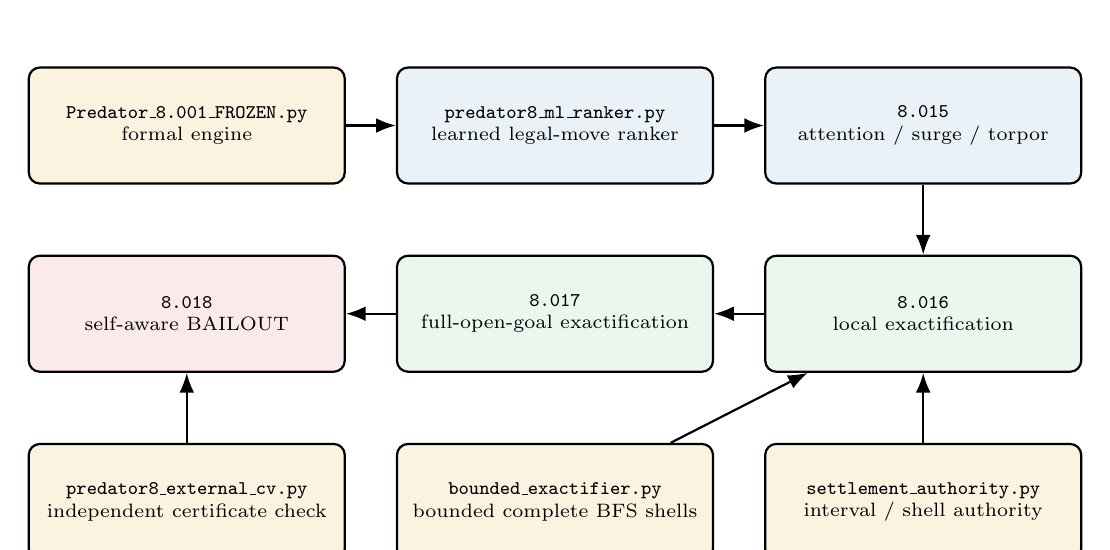
\begin{tikzpicture}[
 box/.style={draw,rounded corners,thick,align=center,font=\scriptsize,minimum width=1.58in,minimum height=0.58in},
 arr/.style={-{Latex[length=2.5mm]},thick}
]
\node[box,fill=softgold] (frozen) {\code{Predator\_8.001\_FROZEN.py}\\formal engine};
\node[box,fill=softblue,right=0.25in of frozen] (rank) {\code{predator8\_ml\_ranker.py}\\learned legal-move ranker};
\node[box,fill=softblue,right=0.25in of rank] (p15) {\code{8.015}\\attention / surge / torpor};
\node[box,fill=softgreen,below=0.35in of p15] (p16) {\code{8.016}\\local exactification};
\node[box,fill=softgreen,left=0.25in of p16] (p17) {\code{8.017}\\full-open-goal exactification};
\node[box,fill=softred,left=0.25in of p17] (p18) {\code{8.018}\\self-aware BAILOUT};
\node[box,fill=softgold,below=0.35in of p17] (exact) {\code{bounded\_exactifier.py}\\bounded complete BFS shells};
\node[box,fill=softgold,right=0.25in of exact] (auth) {\code{settlement\_authority.py}\\interval / shell authority};
\node[box,fill=softgold,left=0.25in of exact] (cv) {\code{predator8\_external\_cv.py}\\independent certificate check};
\draw[arr] (frozen)--(rank); \draw[arr] (rank)--(p15); \draw[arr] (p15)--(p16); \draw[arr] (p16)--(p17); \draw[arr] (p17)--(p18);
\draw[arr] (exact)--(p16); \draw[arr] (auth)--(p16); \draw[arr] (cv)--(p18);
\end{tikzpicture}
\caption{Reconstruction dependency chain. 8.018 wraps the earlier controllers; it does not replace the proof semantics.}
\end{figure}

\subsection{Runtime and data integrity values}

The workflow reconstructs the recovered 8.002 runtime from ten Base64 chunks. Preserve these checks:
\begin{center}
\begin{tabularx}{\textwidth}{>{\raggedright\arraybackslash}p{0.28\textwidth}X}
\toprule
Item & Frozen value \\
\midrule
Recovered runtime Base64 size & \code{167804} bytes \\
Recovered runtime ZIP SHA-256 & \code{92b7fce75efb18a6a50b87729b4c286b14a9e89a94e4c7ffe054f3199252bac3} \\
Historical \code{set.mm} commit & \code{cd577894d8e6bf8b4fe8014c0d525d531507e4b7} \\
\code{set.mm} SHA-256 & \code{1016d7edb0508abde0fe240bb5243e588c5067f8cb10ee6e1cc5733fc05acdb5} \\
Model file & \code{prcom\_quick\_policy.joblib} \\
Model SHA-256 & \code{0531268d3f6b99038d001bfa64bbfebb304620ae7394dc61ca998377cf87884c} \\
Target label & \code{prcom} \\
Target statement & $\vdash\{A,B\}=\{B,A\}$ \\
Random seed & \code{2301} \\
\bottomrule
\end{tabularx}
\end{center}

The workflow enforces no-target-proof leakage: the target proof and downstream material are not supposed to be consumed by the learned search policy.

\section{Predator 8.015 control modes inherited by 8.018}

The recovered 8.002 explorer is the native mode. It is not replaced by $H$ control. In native mode, $\widehat H$ is observation-only in 8.015; higher/lower modes give it limited priority influence.

\begin{center}
\begin{tabular}{llll}
\toprule
Mode & Coordinate & ML weight & $\widehat H$ weight \\
\midrule
native & $(2,3)$ & $1.00$ & $0.00$ \\
high / SURGE & $(3,4)$ & $1.10$ & $0.25$ \\
low / TORPOR & $(1,2)$ & $0.30$ & $0.10$ \\
brute & $(0,0)$ & deterministic fallback & n/a \\
\bottomrule
\end{tabular}
\end{center}

Inherited stagnation thresholds are:
\[
\text{native stale}=1200,\qquad \text{high stale}=1200,\qquad \text{low stale}=2400.
\]
Two meaningful $\widehat H$ improvements close enough together trigger an ATTENTION hold window. In the recovered code the improvement threshold is $0.05$, the attention window is 400 guided expansions, and the hold is 900 guided expansions.

\section{8.016 and 8.017 exactification}

\subsection{Why exactification exists}

The simple $\widehat H$ estimator can claim apparent proximity where none is certified. Therefore a proximity alarm can launch a bounded breadth-first search (BFS) around the snapshot.

The generic exactifier returns either:
\begin{itemize}
\item an exact shell $H=r$ if the first settlement is found in a completely enumerated BFS layer $r$, or
\item a sound lower bound $H\ge d+1$ after completely checking settlement-free shells through $d$ before an expansion/memory cap interrupts the next layer.
\end{itemize}

It never upgrades an incomplete search into an exact claim.

\subsection{The 8.017 correction}

8.016 exactification used the engine's chosen open goal. 8.017 changed only the certification graph: it branches over \emph{every} currently open goal and every assertion-head-compatible candidate that unifies. No learned ranker or opener cap is allowed to prune the certification graph. This is the relevant full-open-goal local geometry.

The important recent lesson was:
\[
\boxed{\widehat H\approx2.03\text{ is not evidence that true }H=2.}
\]
The full graph probe in 8.017 could certify only that the alarming snapshot was not settled at shells 0 or 1 before the next layer became too broad. Therefore $H=2$ remained possible, but so did larger values. That is precisely why a diagnostic probe must have a bailout budget.

\section{Predator 8.018: implemented self-aware bailout}

\subsection{What is genuinely new in the code}

8.018 keeps 8.017's full-open-goal certification graph and substitutes a new guided controller. It introduces:
\begin{itemize}
\item a resource tranche for an active promising basin;
\item basin identity by the first proof-step prefix (currently prefix length 1);
\item a blacklist of failed basin prefixes;
\item frontier pruning of states under blacklisted prefixes;
\item a deliberate switch to high-diversity SURGE after bailout;
\item a diagnostic exactification probe cap tied to the same tranche scale.
\end{itemize}

The first experimental constants are:
\[
\texttt{BAILOUT\_FRACTION}=0.03,\qquad
\texttt{BAILOUT\_MIN\_EXPANSIONS}=250,\qquad
\texttt{BASIN\_PREFIX\_LEN}=1.
\]

Because the 30,000 global budget reserves 6,000 expansions for brute force, the guided controller receives 24,000 expansions. Therefore the initial basin tranche is
\[
\boxed{\lceil0.03\times24{,}000\rceil=720\text{ guided expansions}.}
\]
This 3\% is a tunable hyperparameter, not a theorem constant.

\subsection{Bailout rule as implemented}

Let $b$ be the active basin. A meaningful new best-$\widehat H$ descent resets the basin's resource anchor. If both
\[
R-R_{\mathrm{anchor}}\ge B_{\mathrm{basin}}
\]
and
\[
R-R_{\mathrm{last\ improve}}\ge B_{\mathrm{basin}},
\]
then the controller concludes that it has paid the basin's tranche without useful $\widehat H$ benefit. It then:
\begin{enumerate}
\item adds the basin's prefix to \code{blocked\_prefixes};
\item deletes frontier states whose proof trails begin with that prefix;
\item switches to high/SURGE mode;
\item clears attention and descent-streak state;
\item resumes search among competing branches.
\end{enumerate}

The diagnostic BFS probe is also capped at no more than the basin tranche. This encodes the principle:
\[
\boxed{\text{exactification is a bounded diagnostic, not a second brute-force solver}.}
\]

\subsection{8.018 control flow}

\begin{figure}[H]
\centering
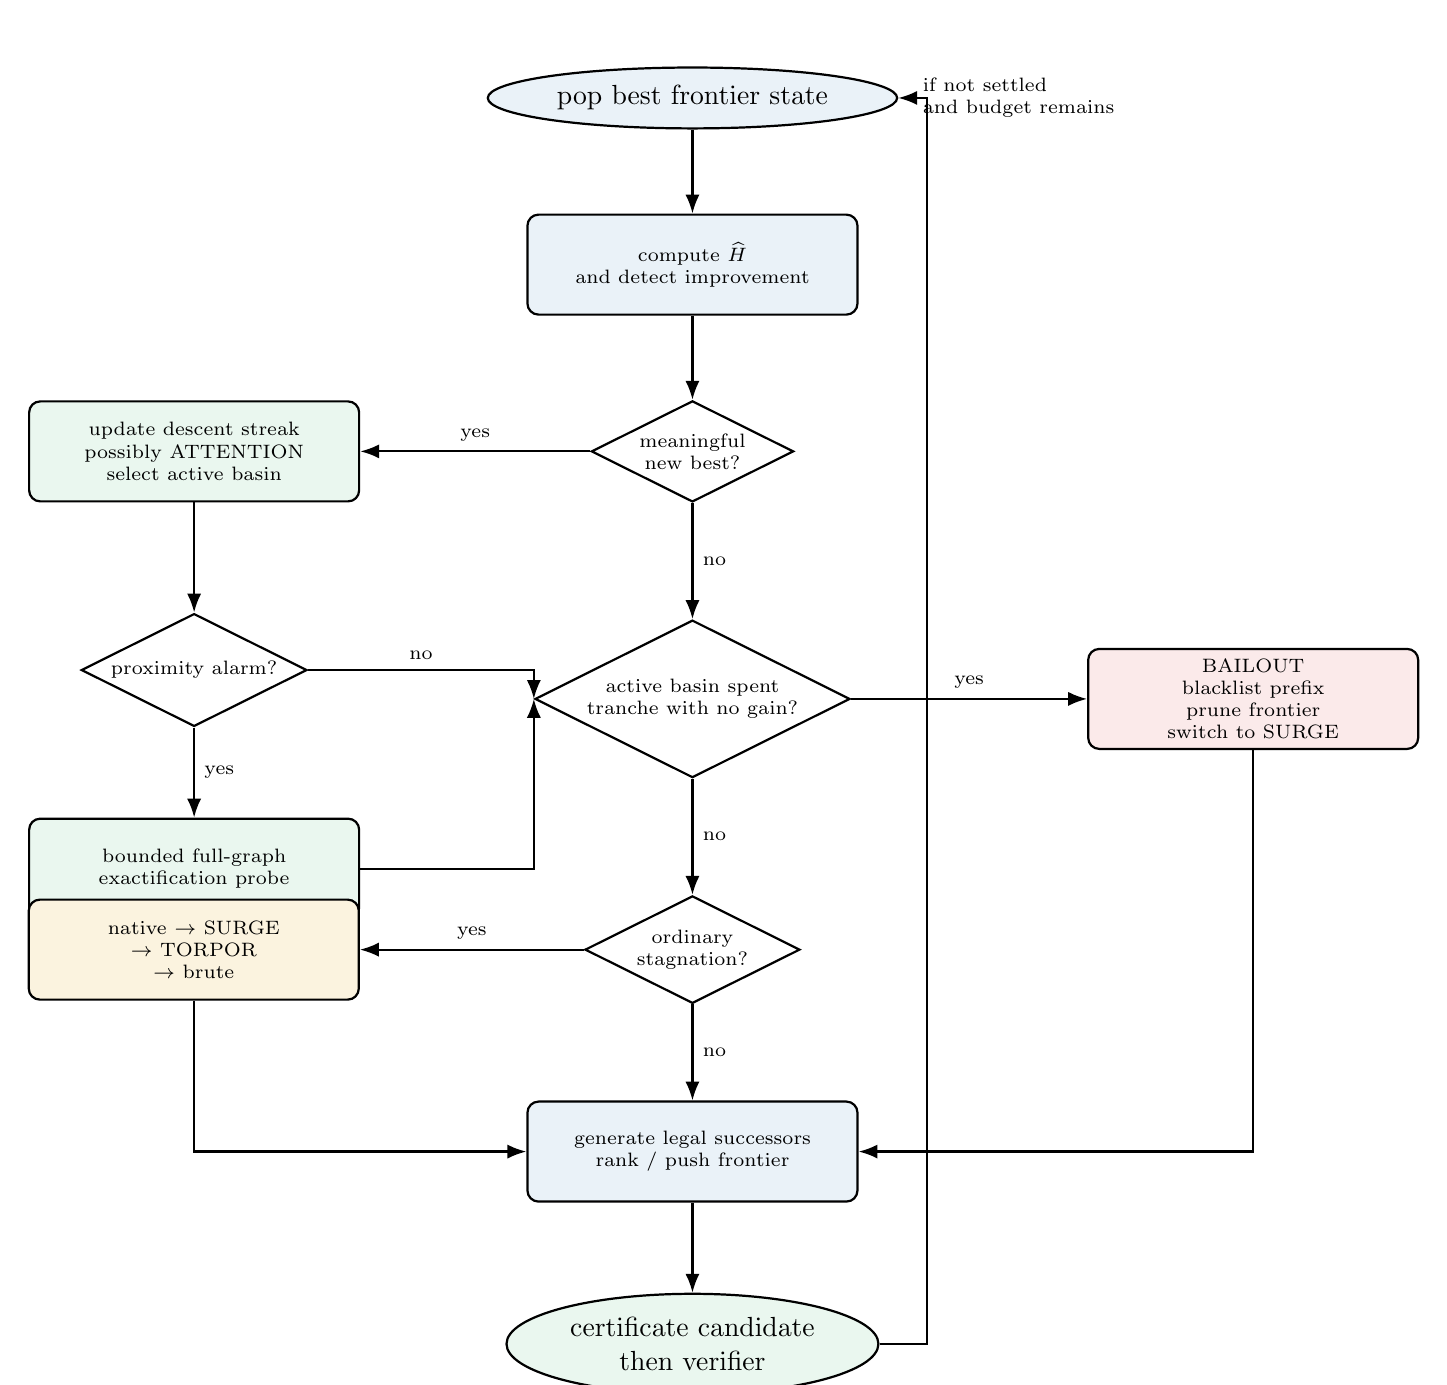
\begin{tikzpicture}[
 node distance=0.42in and 0.55in,
 start/.style={ellipse,draw,thick,fill=softblue,align=center,minimum width=1.4in},
 proc/.style={rectangle,rounded corners,draw,thick,align=center,minimum width=1.65in,minimum height=0.5in,font=\scriptsize},
 dec/.style={diamond,draw,thick,aspect=2.0,align=center,font=\scriptsize,inner sep=1.5pt},
 arr/.style={-{Latex[length=2.4mm]},thick,font=\scriptsize}
]
\node[start] (pop) {pop best frontier state};
\node[proc,fill=softblue,below=of pop] (score) {compute $\widehat H$\\and detect improvement};
\node[dec,below=of score] (imp) {meaningful\\new best?};
\node[proc,fill=softgreen,left=1.15in of imp] (att) {update descent streak\\possibly ATTENTION\\select active basin};
\node[dec,below=0.55in of att] (probeq) {proximity alarm?};
\node[proc,fill=softgreen,below=0.45in of probeq] (probe) {bounded full-graph\\exactification probe};
\node[dec,below=0.58in of imp] (bailq) {active basin spent\\tranche with no gain?};
\node[proc,fill=softred,right=1.18in of bailq] (bail) {BAILOUT\\blacklist prefix\\prune frontier\\switch to SURGE};
\node[dec,below=0.58in of bailq] (stale) {ordinary\\stagnation?};
\node[proc,fill=softgold,left=1.12in of stale] (modes) {native $\to$ SURGE\\$\to$ TORPOR\\$\to$ brute};
\node[proc,fill=softblue,below=0.48in of stale] (expand) {generate legal successors\\rank / push frontier};
\node[start,fill=softgreen,below=0.45in of expand] (settle) {certificate candidate\\then verifier};

\draw[arr] (pop)--(score); \draw[arr] (score)--(imp);
\draw[arr] (imp)--node[above]{yes}(att); \draw[arr] (imp)--node[right]{no}(bailq);
\draw[arr] (att)--(probeq); \draw[arr] (probeq)--node[right]{yes}(probe); \draw[arr] (probe.east) -| (bailq.west);
\draw[arr] (probeq.east) -| node[pos=0.25,above]{no} (bailq.west);
\draw[arr] (bailq)--node[above]{yes}(bail); \draw[arr] (bail.south) |- (expand.east);
\draw[arr] (bailq)--node[right]{no}(stale); \draw[arr] (stale)--node[above]{yes}(modes); \draw[arr] (modes.south) |- (expand.west);
\draw[arr] (stale)--node[right]{no}(expand); \draw[arr] (expand)--(settle);
\draw[arr] (settle.east) -- ++(0.6,0) |- node[pos=0.75,right,align=left]{if not settled\\and budget remains} (pop.east);
\end{tikzpicture}
\caption{Current 8.018 control flow. BAILOUT is based on resource spent without new best-$\widehat H$ benefit.}
\end{figure}

\section{Current 30k experiment configuration}

The GitHub workflow invokes 8.018 with:
\begin{lstlisting}
--label prcom
--budget 30000
--brute-reserve 6000
--max-depth 12
--max-open 8
--seed 2301
--creativity 0.55
--opener-cap 48
--progress 250
--frontier-limit 120000
--probe-depth 3
--probe-cap 2000
--probe-total-cap 4000
--probe-next-layer 30000
\end{lstlisting}

The output candidate, if any, is \code{prcom\_p8\_018.mm}. It is checked by the external certificate verifier. The workflow artifact is intended to contain hashes, authority tests, root-rank diagnostics, controller logs, return code, independent CV log, and emitted proof if one exists.

\subsection{Run to check first on restart}

At this snapshot:
\begin{center}
\begin{tabular}{ll}
\toprule
GitHub Actions run & \code{32966066334} \\
Workflow & \code{Predator8 prcom self-aware bailout} \\
Commit & \code{77aad00387b459b05da35abaea5e43d2fbd0a6db} \\
Status at note freeze & \textbf{in progress} \\
\bottomrule
\end{tabular}
\end{center}

\textbf{Restart instruction:} before changing any code, fetch this run's final jobs/logs/artifact. Record whether BAILOUT actually fired, which basin prefix was blocked, how many frontier states were pruned, whether another $\widehat H$ improvement occurred afterward, total guided/probe/brute allocation, and whether a verified certificate was emitted.

\section{Mathematical results already developed but not fully implemented}

\subsection{Discrete Settlement Convergence Theorem}

Let $(x_t)$ be a trajectory in a unit-cost settlement graph with finite initial horizon. If whenever $H(x_t)>0$ the controller chooses an admissible successor with
\[
H(x_{t+1})<H(x_t),
\]
then, since $H$ is integer-valued,
\[
H(x_{t+1})\le H(x_t)-1.
\]
Therefore settlement occurs in finite time:
\[
\boxed{\tau_0\le H(x_0).}
\]
If every selected edge is geodesic, then
\[
\boxed{H(x_t)=H(x_0)-t,\qquad \tau_0=H(x_0).}
\]
This theorem is a global finite-capture consequence of Proof Compass-style local navigation. 8.018 does not enforce exact $H$ descent because it does not know exact $H$ globally.

\subsection{Half-Step Controlled Settlement}

If true successor horizons are integers and a certified estimator satisfies
\[
|\widehat H(y)-H(y)|<\frac12
\]
for every candidate successor $y$, then greedy minimization of $\widehat H$ preserves the ordering of distinct horizon shells and selects a true geodesic successor. Combined with discrete convergence, this gives shortest-path finite settlement.

Do \textbf{not} implement this as a guarantee unless the $<1/2$ error bound is actually certified. The present heuristic demonstrably does not satisfy such a guarantee everywhere.

\subsection{Certified Near-Zero Saturation}

Under the same half-step guarantee,
\[
\widehat H(x)<m+\frac12\quad\Rightarrow\quad H(x)\le m.
\]
If branching is finite, complete local saturation to depth $m$ must then encounter settlement. This yields a useful architecture split:
\[
\boxed{\text{navigate globally} \to \text{enter a certified small shell} \to \text{saturate locally} \to H=0.}
\]
This is not yet implemented as a distinct SATURATE mode.

\subsection{The new self-awareness principle}

The theoretical Level-3 question is:
\[
\boxed{\text{Am I putting in cost and cost and cost while getting little or no settlement benefit?}}
\]
If yes for long enough, change strategy. 8.018 implements only a crude version based on ``no new best $\widehat H$ over a fixed tranche.'' The fuller theory should evaluate progress, certified information, and cost together.

\section{Selective kitchen-sink roadmap: what should be added next}

The next version should include only mechanisms with an obvious path to saving expansions or finding settlement. It should \emph{not} turn mathematical theory into decorative code.

\subsection{Include}

\begin{enumerate}
\item \textbf{Adaptive BAILOUT.} Replace a permanently fixed 3\% with a bounded patience parameter that can be tuned across runs and, later, learned by strategy/basin type.
\item \textbf{$H$-velocity.}
\[
v_H=-\frac{\Delta\widehat H}{\Delta R}.
\]
Use a smoothed short-window estimate. Positive $v_H$ means apparent movement toward settlement.
\item \textbf{Trend / acceleration signal.}
\[
a_H=-\frac{\Delta^2\widehat H}{\Delta R^2}.
\]
Use only as a trend detector; do not let noisy second differences dominate control.
\item \textbf{Certified information gain.} Track sound horizon information such as $H\in[L,U]$. Reward genuine interval tightening. Repeating $[2,\infty)$ after spending another tranche should yield essentially zero information benefit.
\item \textbf{SATURATE versus BAILOUT.} A low $\widehat H$ basin should receive intensive local search only if evidence is still improving. Low $\widehat H$ plus stagnant evidence should trigger bailout.
\item \textbf{Multiple live basins.} Maintain a small portfolio rather than allowing one basin to monopolize the search. Allocate resource tranches across competitors.
\item \textbf{Resource/benefit accounting per basin and strategy.} Estimate utility per cost rather than absolute attractiveness alone.
\item \textbf{$\tau_0$ telemetry.} First verified settlement resource must be the ultimate experimental score.
\item \textbf{Strategy memory.} Remember failed basins/strategies so the controller does not repeatedly re-enter the same quicksand.
\end{enumerate}

\subsection{Do not add yet}

For the immediate \code{prcom} experiment, leave out anything obviously unhelpful:
\begin{itemize}
\item NSA as a runtime ``mode''; NSA belongs to the mathematical analysis of search dynamics here.
\item Hypernatural/hyperfinite machinery in Python merely for terminology.
\item Any false assumption that half-step accuracy already holds.
\item Full $P/R/I/C$ AMLD role expansion for a target already known to be a theorem.
\item Coupled-pair catalysis unless the experiment is explicitly switched back to the multi-agent AMLD system.
\item Complex learned hyperparameter optimization before enough runs exist to learn from.
\item Additional metrics that duplicate a simpler signal without a clear decision use.
\end{itemize}

\section{Proposed next controller: selective kitchen sink}

\subsection{State to maintain per basin}

For each live basin $b$, maintain a record conceptually like:
\begin{lstlisting}
BasinRecord:
    prefix / basin_id
    active_frontier_count
    total_resource_spent
    tranche_resource_spent
    best_h_hat
    h_hat_history_window
    v_h_smoothed
    a_h_smoothed
    certified_lower_bound L
    certified_upper_bound U (if any)
    information_gain_history
    last_progress_resource
    bailout_count / reentry_penalty
    status = EXPLORE | ATTEND | SATURATE | SURGE | TORPOR | BLOCKED
\end{lstlisting}

The Professor keeps a small set of live basin records plus a blocked/retired memory.

\subsection{Useful, deliberately simple utility}

A first non-learned utility should be transparent:
\[
U_b=
\frac{
\alpha\,\Delta H_{\mathrm{benefit}}
+\beta\,\Delta I_{\mathrm{cert}}
+\gamma\,\Delta C_{\mathrm{completion}}
+\eta\,N_{\mathrm{novelty}}
}{\Delta R+\varepsilon}.
\]
Interpretation:
\begin{itemize}
\item $\Delta H_{\mathrm{benefit}}$: smoothed improvement in $\widehat H$ or other calibrated settlement proxy;
\item $\Delta I_{\mathrm{cert}}$: sound tightening of $[L,U]$ or stronger verifier-relevant evidence;
\item $\Delta C_{\mathrm{completion}}$: direct completion progress, especially closed/near-closed proof states;
\item $N_{\mathrm{novelty}}$: modest reward for exploring a genuinely distinct basin after stagnation;
\item $\Delta R$: resource consumed.
\end{itemize}
The weights are hyperparameters. Start simple; log everything; tune from observed behavior rather than pretending the first weights are theoretically privileged.

\subsection{Decision rule}

The key distinction should be:
\[
\boxed{
\begin{array}{ll}
\widehat H\text{ low} + \text{new useful evidence arriving}
&\Rightarrow \text{SATURATE / continue},\\[1mm]
\widehat H\text{ low} + \text{no useful evidence arriving}
&\Rightarrow \text{BAILOUT},\\[1mm]
\widehat H\text{ not low} + v_H>0
&\Rightarrow \text{continue navigation},\\[1mm]
\widehat H\text{ not low} + v_H\approx0
&\Rightarrow \text{SURGE / diversify / switch basin}.
\end{array}}
\]

\subsection{Suggested state machine}

\begin{figure}[H]
\centering
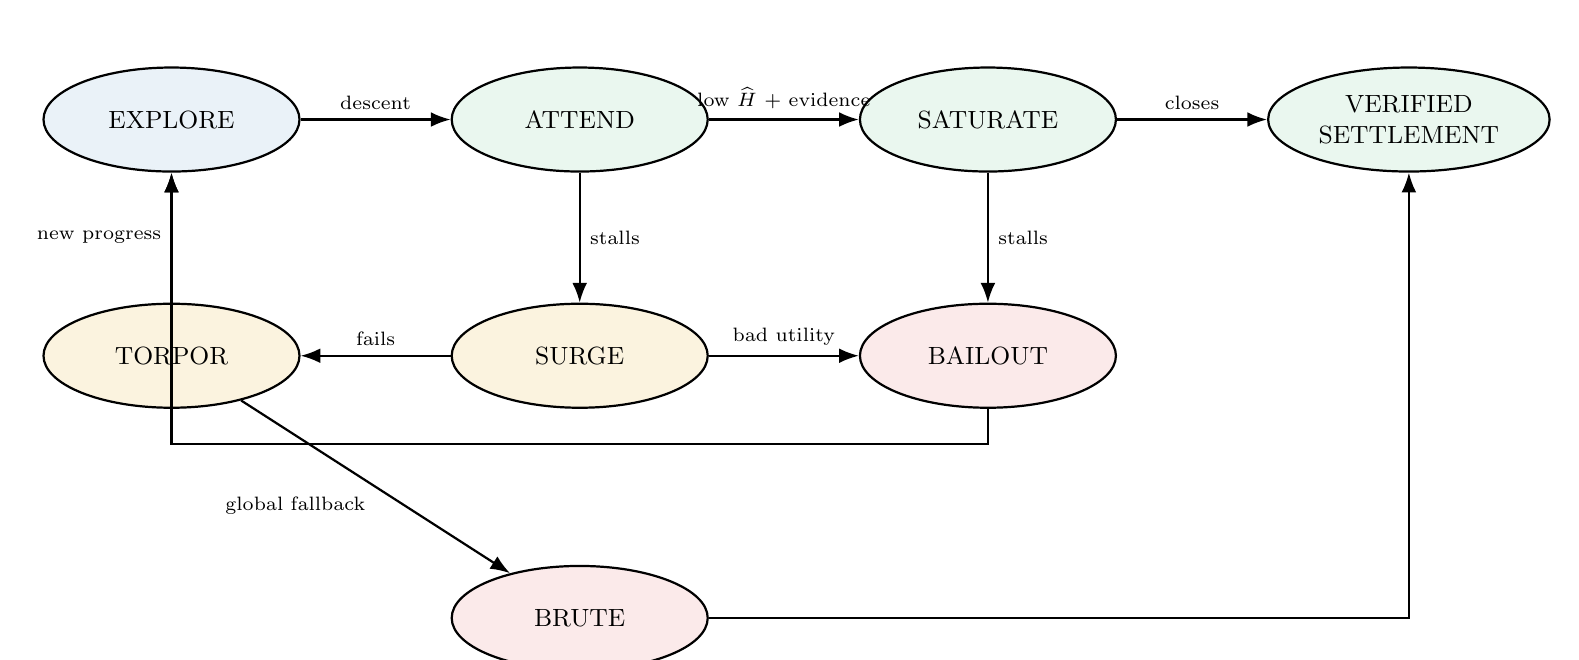
\begin{tikzpicture}[
 st/.style={ellipse,draw,thick,align=center,minimum width=1.28in,minimum height=0.52in,font=\small},
 arr/.style={-{Latex[length=2.5mm]},thick,font=\scriptsize},
 node distance=0.65in and 0.75in
]
\node[st,fill=softblue] (explore) {EXPLORE};
\node[st,fill=softgreen,right=of explore] (attend) {ATTEND};
\node[st,fill=softgreen,right=of attend] (sat) {SATURATE};
\node[st,fill=softgreen,right=of sat] (settle) {VERIFIED\\SETTLEMENT};
\node[st,fill=softgold,below=of attend] (surge) {SURGE};
\node[st,fill=softgold,left=of surge] (torpor) {TORPOR};
\node[st,fill=softred,right=of surge] (bail) {BAILOUT};
\node[st,fill=softred,below=0.78in of surge] (brute) {BRUTE};

\draw[arr] (explore)--node[above]{descent}(attend);
\draw[arr] (attend)--node[above]{low $\widehat H$ + evidence}(sat);
\draw[arr] (sat)--node[above]{closes}(settle);
\draw[arr] (attend)--node[right]{stalls}(surge);
\draw[arr] (surge)--node[above]{fails}(torpor);
\draw[arr] (torpor)--node[left]{new progress}(explore);
\draw[arr] (surge)--node[above]{bad utility}(bail);
\draw[arr] (sat)--node[right]{stalls}(bail);
\draw[arr] (torpor)--node[below left]{global fallback}(brute);
\draw[arr] (brute) -| (settle.south);
\draw[arr] (bail.south) -- ++(0,-0.45) -| (explore.south);
\end{tikzpicture}
\caption{Proposed selective kitchen-sink controller. The critical new branch is the distinction between earned local saturation and quicksand bailout.}
\end{figure}

\section{Pseudocode for the next implementation}

\begin{lstlisting}
initialize proof frontier
initialize basin portfolio and blocked-basin memory
initialize global resource budget B

while budget remains and no verified settlement:
    choose a basin b by expected utility per resource
    choose/pop a proof state q inside b
    expand one legal proof move using current mode/profile
    update h_hat telemetry for b
    update smoothed v_h and trend/acceleration

    if proof closes:
        emit candidate
        if verifier ACCEPTS:
            record tau_0 and stop

    if descent/proximity alarm fires:
        spend only a bounded diagnostic tranche on exactification
        update sound interval [L_b, U_b]
        compute certified information gain

    benefit = weighted(
        h_hat improvement,
        certified interval tightening,
        completion evidence,
        modest novelty
    )
    utility = benefit / resource_spent

    if certified small shell and evidence continues to improve:
        SATURATE locally within a separately bounded tranche
    elif tranche exhausted and utility is near zero:
        BAILOUT:
            block or heavily penalize basin b
            prune/deprioritize its frontier
            switch to a competing basin / diversify
    elif progress has slowed but basin remains plausible:
        SURGE or change search profile
    elif surge fails:
        TORPOR / coverage mode

if no guided basin remains worth funding:
    use declared bounded brute fallback

never treat h_hat, utility, or self-awareness as theorem authority
\end{lstlisting}

\section{Telemetry needed to make the theory empirical}

Every run should emit a machine-readable event stream sufficient to reconstruct decisions. At minimum log:
\begin{itemize}
\item global expansion/resource count;
\item active basin ID/prefix and mode;
\item current/best $\widehat H$;
\item smoothed $v_H$ and trend signal;
\item last sound interval $[L,U]$ and how it was obtained;
\item exactification expansions spent and whether the requested shell was complete;
\item information gain credited to a probe;
\item basin resource spent since last progress;
\item utility estimate used to continue, surge, saturate, or bail;
\item BAILOUT events and number of frontier states pruned;
\item basin reentry attempts/penalties;
\item final guided/probe/brute totals;
\item first certificate candidate resource;
\item independent verifier result;
\item $\tau_0$ if settled.
\end{itemize}

A recommended event schema is:
\begin{lstlisting}
EVENT, R_total, R_guided, R_probe, basin_id, mode,
h_hat, best_h_hat, v_h, a_h, L, U,
probe_complete, info_gain, basin_spent, utility,
decision, frontier_size, blocked_count
\end{lstlisting}

\section{How to interpret ``quicksand'' mathematically}

A time basin is not merely a branch with a bad absolute score. It is a region in which additional resource yields little marginal settlement benefit. The primitive empirical signature is:
\[
\frac{\Delta\text{benefit}}{\Delta R}\approx0
\quad\text{over a bounded window.}
\]
Useful benefit may include:
\[
-\Delta\widehat H>0,\qquad
\Delta I_{\mathrm{cert}}>0,\qquad
\text{or direct completion/verifier evidence}.
\]
Thus the future rule should be stronger than ``stuck near 2.'' It should be:
\[
\boxed{\text{large continuing cost + negligible marginal benefit} \Rightarrow \text{strategy evidence: leave}.}
\]
This turns self-awareness from a label into a measurable feedback mechanism.

\section{What remains outside this single-prover experiment}

The broader AMLD architecture is richer than Predator 8.018. Important concepts to retain for later, but not force into the current \code{prcom} run, include:
\begin{itemize}
\item four settlement channels $P,R,I,C$ with verifier $V$;
\item role-specific horizons $(H_P,H_R,H_I,H_C)$ and overall $H_{\mathrm{AMLD}}=\min(H_P,H_R,H_I,H_C)$;
\item coupled role pairs $(P_1,P_2)$, $(R_1,R_2)$, $(I_1,I_2)$, $(C_1,C_2)$;
\item pair-state settlement geometry and catalysis/synergy measures;
\item shared verified BANK, tentative workspaces, and partner state/advice communication;
\item Professor resource allocation across role pairs;
\item nonstandard-analysis results about hyperfinite search dynamics, which are theory about the search space rather than a runtime heuristic.
\end{itemize}

These should be reintroduced when the experiment returns to genuine AMLD multi-settlement tasks.

\section{Banked-settlement sanity test to run later}

Do \textbf{not} use this in the current 8.018 experiment. But retain the planned architecture test:
\begin{enumerate}
\item Give the AMLD a target $c$.
\item Put a verified certificate/provenance pair $(c,\pi_c)$ in BANK.
\item Require the architecture to retrieve and submit it to $V$.
\item Expect settlement in approximately $O(1)$ architecture steps (exact count depends on whether retrieval/submission and verifier acceptance are modeled as separate graph edges).
\end{enumerate}
If the system takes thousands of expansions or returns UNKNOWN in that setup, the architecture is failing to exploit known settlement information. Only after the architecture passes this sanity test should increasingly incomplete proofs be placed in BANK to calibrate operational $H=1,2,3,\ldots$ shells.

\section{Resume procedure after loss of context}

Use this sequence exactly enough to avoid silently changing the experiment.

\begin{enumerate}
\item \textbf{Check out the reconstruction commit} \code{77aad00387b459b05da35abaea5e43d2fbd0a6db} or inspect the diff from it before using a later commit.
\item \textbf{Recover the runtime} from \code{predator 8/recovered8\_002/runtime\_chunks/part00.b64} through \code{part09.b64}; verify Base64 size and runtime ZIP hash listed above.
\item \textbf{Recover the exact environment} \code{set.mm} at commit \code{cd577894...}; verify its SHA-256.
\item \textbf{Recover the model} \code{prcom\_quick\_policy.joblib}; verify its SHA-256.
\item \textbf{Run the theorem-authority integration tests} before trusting any exactification result.
\item \textbf{Fetch final result of Actions run 32966066334}. Save logs/artifact before modifying code.
\item \textbf{Record whether 8.018 actually improved behavior} relative to 8.016/8.017: number/timing of bailouts, alternate basin progress, total time, and settlement status.
\item If continuing tonight's design direction, implement the selective kitchen-sink controller in a \textbf{new version} (suggested \code{8.019}), preserving 8.018 unchanged for ablation/reproducibility.
\item Keep the exact same \code{prcom} target, model, seed, environment, global budget, and proof/verifier semantics for the first 8.019 comparison unless explicitly designing another experiment.
\item Add one decision mechanism at a time in code, but the first kitchen-sink run may enable the whole selected set; later use ablations to attribute any gain.
\end{enumerate}

\section{Failure diagnosis table}

\begin{longtable}{p{0.25\textwidth}p{0.32\textwidth}p{0.36\textwidth}}
\toprule
Observed symptom & Likely interpretation & Next check/action \\
\midrule
\endfirsthead
\toprule
Observed symptom & Likely interpretation & Next check/action \\
\midrule
\endhead
$\widehat H$ drops then stalls, no stronger exact evidence & Heuristic basin may be quicksand & Bail out after bounded tranche; do not exhaust local BFS \\
Exactifier repeatedly returns same $[L,\infty)$ & Little/no information gain & Stop funding probe/basin unless other progress exists \\
Exactifier finds exact small $H$ or tight finite upper bound & Genuine near-settlement evidence & Enter bounded SATURATE/completion mode \\
BAILOUT fires but frontier quickly re-enters same structure & Basin identity too shallow or reentry penalty too weak & Increase prefix representation or add structural basin signature \\
No basin ever earns ATTENTION & $\widehat H$ signal too weak/noisy or thresholds too strict & Inspect raw $\widehat H$ trace; tune improvement/window parameters \\
Many bailouts with no later progress & Controller is switching but not generating better alternatives & Improve basin portfolio/diversity, not just lower bailout threshold \\
Brute force consumes most budget again & Guided metacontrol failed to produce useful alternatives soon enough & Compare guided utility and bailout timing; reconsider reserve allocation only after diagnosis \\
Certificate candidate appears but verifier rejects & Protocol/proof reconstruction defect & Treat as failure; debug emitter/verifier boundary before search heuristics \\
Banked-settlement sanity test is slow & Architecture/retrieval failure & Fix BANK routing before judging $H$ navigation \\
\bottomrule
\end{longtable}

\section{Experiment comparison sheet}

Fill this table as versions finish; do not rely on memory.

\begin{center}
\begin{tabularx}{\textwidth}{lrrrrX}
\toprule
Version & Budget & Guided+probe & Brute & Best $\widehat H$ & Result / key diagnosis \\
\midrule
8.016 & 30k & 5,017 & 24,983 & 2.030 & UNKNOWN; local restricted probe certified $H\ge3$ and denied half-gap proximity \\
8.017 & 30k & 4,948 & 25,052 & 2.030 & UNKNOWN; full-open-goal probe only certified $H\ge2$ before shell explosion \\
8.018 & 30k & -- & -- & -- & \textbf{fill from run 32966066334}; self-aware basin bailout \\
8.019 proposed & 30k & -- & -- & -- & selective kitchen sink: adaptive utility, SATURATE vs BAILOUT, basin portfolio \\
\bottomrule
\end{tabularx}
\end{center}

\section{Research claims versus engineering hypotheses}

Keep these categories separate on restart.

\subsection*{Mathematical statements already proved under stated hypotheses}
\begin{itemize}
\item integer-valued unit settlement horizon has isolated zero;
\item strict exact-$H$ descent implies finite settlement;
\item geodesic descent gives $H_t=H_0-t$;
\item certified error $<1/2$ recovers integer horizon shell and preserves geodesic ordering;
\item certified entry into a finite near-zero shell plus complete local saturation implies settlement.
\end{itemize}

\subsection*{Engineering hypotheses to test}
\begin{itemize}
\item $\widehat H$ descent is useful enough to trigger attention;
\item resource/benefit self-awareness saves search budget;
\item basin bailout finds better alternatives than prolonged local persistence;
\item information-gain accounting improves the stay/leave decision;
\item multiple-basin resource allocation lowers $\tau_0$;
\item selective near-zero saturation outperforms either always-saturate or always-bail behavior.
\end{itemize}

\section{Compact reconstruction specification}

If only one page of these notes is remembered, reconstruct the controller from this specification:

\begin{quote}
Start with the recovered Predator 8.002 legal proof engine and ML ranker, under strict pre-target theorem cutoff and external Metamath verification. Use the simple $\widehat H$ only as non-authoritative search telemetry. Keep native recovered search when $\widehat H$ is improving; use bounded exactification to test apparent proximity; never let exactification become a second brute-force search. Track proof-tree basins. A basin earns a resource tranche only while it produces settlement progress or new certified information. If cost accumulates with negligible benefit, BAILOUT: suppress that basin, preserve its failure memory, and deliberately allocate search elsewhere. Distinguish low-$\widehat H$ basins that continue to generate evidence (SATURATE) from low-$\widehat H$ basins that merely consume time (BAILOUT). Judge the experiment by first verified settlement resource $\tau_0$, not by heuristic values. All self-awareness and Professor decisions remain subordinate to the verifier.
\end{quote}

\section{Final checkpoint}

The conceptual checkpoint at document freeze is:
\[
\boxed{
\begin{array}{c}
\text{Level 1: choose legal proof moves}\\
\downarrow\\
\text{Level 2: ask whether settlement distance/evidence is improving}\\
\downarrow\\
\text{Level 3: ask whether the strategy is worth its ongoing cost}\\
\downarrow\\
\text{continue, saturate, surge, torpor, bail out, or switch}\\
\downarrow\\
\text{verified settlement is the only success condition.}
\end{array}}
\]

The immediate next empirical task is to read the final 8.018 run, not to assume success or failure. The immediate next engineering task, if the bailout experiment supports the idea, is a new selective kitchen-sink version that adds only obviously useful metacognitive signals: adaptive patience, smoothed settlement velocity/trend, certified information gain, SATURATE-versus-BAILOUT, multiple live basins, strategy memory, and explicit $\tau_0$ telemetry.

\appendix
\section{Named files needed for reconstruction}

\begin{itemize}
\item \code{predator 8/recovered8\_002/Predator\_8.001\_FROZEN.py}
\item \code{predator 8/recovered8\_002/predator8\_ml\_ranker.py}
\item \code{predator 8/recovered8\_002/predator8\_external\_cv.py}
\item \code{predator 8/recovered8\_002/setmm\_grammar.py}
\item \code{predator 8/recovered8\_002/metamath.py}
\item \code{predator 8/recovered8\_002/prcom\_quick\_policy.joblib}
\item \code{predator 8/recovered8\_002/predator8\_015\_bidirectional\_attention.py}
\item \code{predator 8/recovered8\_002/predator8\_016\_prcom\_exactify.py}
\item \code{predator 8/recovered8\_002/predator8\_017\_fullgraph\_exactify.py}
\item \code{predator 8/recovered8\_002/predator8\_018\_bailout.py}
\item \code{predator 8/recovered8\_002/bounded\_exactifier.py}
\item \code{predator 8/recovered8\_002/settlement\_authority.py}
\item \code{predator 8/recovered8\_002/predator8\_authority\_adapter.py}
\item \code{predator 8/recovered8\_002/\_loss.py}
\item \code{predator 8/recovered8\_002/runtime\_chunks/part00.b64} through \code{part09.b64}
\item \code{.github/workflows/predator8-prcom-bailout.yml}
\end{itemize}

\section{Source provenance for these notes}

These notes were reconstructed from the active research discussion and the repository snapshot named on the title page. In particular, the implementation details were checked against the current 8.015, 8.016, 8.017, 8.018 controller files and the 8.018 GitHub Actions workflow. The theory-only sections intentionally preserve the distinction between proved statements and proposed controller mechanisms.

\end{document}
